\documentclass[10pt,conference,compsocconf]{IEEEtran}

\usepackage{xcolor}
\usepackage{hyperref}
\usepackage{graphicx}	% For figure environment
\usepackage{amsmath}
\usepackage{booktabs}

% Accent colour for links, the same blue as in the plots
\definecolor{accent}{HTML}{2A78D6}
\hypersetup{colorlinks=true, linkcolor=accent, citecolor=accent, urlcolor=accent}


\raggedbottom  % no stretched gaps between paragraphs
\setlength{\textfloatsep}{10pt plus 2pt minus 2pt}  % less space between the floats and the text

\begin{document}
\title{Predicting Coronary Heart Disease\\from Health Survey Answers}

\author{
  Timo Fischer, Alexandre Pestel, Herman Kristiansen\\
  \textit{CS-433 Machine Learning, EPFL, Switzerland, 27 October 2026}\\
  \{timo.fischer, alexandre.pestel, herman.kristiansen\}@epfl.ch
}

\maketitle

\begin{abstract}
  Heart disease is one of the leading causes of death, and finding the people
  at risk early helps prevent it. From the answers to a large U.S. health
  survey, we predict whether a person has been diagnosed with coronary heart
  disease, using only methods we implemented ourselves. Since fewer than one
  in ten people has the disease, we use the F1 score, which rewards finding
  the sick rather than simply being right most of the time. Logistic regression is the best of the basic methods, and it is held back
  by being too simple rather than by a lack of data. Combinations of
  known risk factors improve it, and averaging it with gradient boosted trees
  gives an F1 score of 0.436 in cross-validation and 0.447 on the test set.
  We also found and left out a question that gives the answer away.
\end{abstract}

\section{Introduction}

The BRFSS is a U.S. telephone survey, in which people answer questions about
their health and lifestyle~\cite{brfss15}. From these answers, we predict
whether a person has been told by a doctor that they have coronary heart
disease (MICHD). Each person gives 321 answers, ranging from age and smoking
habits to earlier diagnoses such as stroke or diabetes, but almost half of
all answers are missing. We have 328,135 people for training and 109,379 for
testing.

Only 8.8\% of the people are sick, so a model that calls everyone healthy is 91\% right and still useless. We therefore use the F1 score,
which combines precision and recall.

\section{Models and Methods}

\subsection{Data Preparation}

We clean the data in four steps. First, we drop 18
columns that describe the interview rather than the person, such as the
state, the date and the survey weights. We also drop the raw height and
weight, which mix units, since the survey already provides them in kilograms
and metres together with the BMI. Second, the survey stores answers such as ``don't know'' and ``refused'' as
special numbers, for example 7 and 9 or 77 and 99 depending on the question,
and ``none'' as 88 or 888. Left as they are, these codes would look like very
large answers, so we turn the first ones into missing values and ``none''
into 0. We recognize the format of each question from its largest value,
which works for 233 of the 301 remaining columns. Third, 99 columns are empty for more than nine out of ten people, mostly
follow-up questions that were only asked to a sub-group such as diabetics.
The linear models drop them, while the trees keep them because whether a
person answered a question is itself informative. Finally, the linear models need complete inputs on a common scale. We fill
the remaining gaps with the median of each column, drop the 4 columns that are
then constant and rescale the others to mean 0 and standard deviation 1, so
that years, kilograms and days become comparable. This leaves 198 inputs.

\subsection{Models}

We start with the six basic methods we implemented. Four are forms of linear
regression, which treat the label (0 for healthy and 1 for
sick) as a number to fit. Least squares and ridge regression find the best
fit directly, while gradient descent (GD) and stochastic gradient descent
(SGD, one person at a time) approach it step by step.
The other two are logistic regression, with and without a penalty on
large weights, which instead predicts the probability of being sick. We also
add a linear support vector machine (SVM).

All of these models give each answer a fixed weight and add up the
contributions. Ten extra years must then count the same at 30 as at 70, and
smoking cannot count more for a person who also has diabetes. To allow such
effects in logistic regression, we add the square of every answer with more
than two values and the product of every pair among 20 known risk factors,
such as age, weight, blood pressure, smoking and diabetes. These new inputs
are closely related, which makes gradient descent learn too slowly, so we use Newton's method, which takes fewer and better-aimed steps.

Finally, we implement gradient boosted trees~\cite{xgboost}. Each tree asks a few yes/no
questions, such as whether the person is over 65, and each new tree corrects
the mistakes of the trees before it. Our final model averages the
probabilities predicted by the trees and by logistic regression.

\subsection{Evaluation}

We measure every model by 5-fold cross-validation (CV). The training data is
split into five parts, and each part is predicted by a model trained on the
other four. Since sick people are rare, a probability above 0.5 almost never
occurs, so we choose the cut-off that gives the best F1 on all five parts
together, then score each part with it. All models use the same five parts, so we can compare them part by part and
see whether a small gain is real or due to chance.

\emph{Settings.} Weights start at zero, and every penalty uses
$\lambda = 10^{-4}$. Gradient descent runs 500 steps of size $1/L$, the
largest that still guarantees progress, where $L$ is the largest eigenvalue
of $X^\top X/N$, divided by 4 for logistic regression. SGD takes one step of
size $10^{-5}$ per person, since larger steps diverge. The SVM runs
500 steps of size $1/\sqrt{t}$, the weighted SVM makes each class count for
half of the loss, and Newton's method runs 10 steps. Values are capped at
$\pm 5$ before squaring. The boosting uses 250 trees of depth 4, each built
on 70\% of the people drawn without replacement and added with weight 0.1.
The cut-off is one of $0.05, 0.06, \dots, 0.95$, and all random draws use
seed 42.

\section{Results}

\subsection{Comparison of the Linear Methods}

Logistic regression is the best of the six methods (Table~\ref{tab:linear}).
Linear regression is penalized even for predictions that are too confident,
such as 1.4 for a sick person, which pulls it away from the hard cases.
The SVM does poorly unless sick people are given more weight, because calling everyone healthy is already almost optimal for it, and even
with weights it stays behind logistic regression.

\begin{table}[tbp]
  \centering
  \caption{The six basic methods and the SVM in 5-fold CV. $\Delta$F1 is the
  part-by-part difference with the reference.}
  \label{tab:linear}
  \footnotesize
  \begin{tabular}{lcc}
    \toprule
    Method & F1 & $\Delta$F1 \\
    \midrule
    Least squares          & $0.418 \pm 0.003$ & $-0.008 \pm 0.002$ \\
    Ridge regression       & $0.418 \pm 0.003$ & $-0.008 \pm 0.002$ \\
    Linear regression, GD  & $0.418 \pm 0.003$ & $-0.007 \pm 0.002$ \\
    Linear regression, SGD & $0.412 \pm 0.004$ & $-0.013 \pm 0.004$ \\
    Logistic, no penalty   & $0.425 \pm 0.002$ & $\phantom{-}0.000 \pm 0.000$ \\
    Logistic, with penalty & $\mathbf{0.425 \pm 0.002}$ & reference \\
    SVM                    & $0.402 \pm 0.009$ & $-0.024 \pm 0.010$ \\
    SVM, weighted          & $0.424 \pm 0.003$ & $-0.002 \pm 0.001$ \\
    \bottomrule
  \end{tabular}
\end{table}

\begin{figure}[tbp]
  \centering
  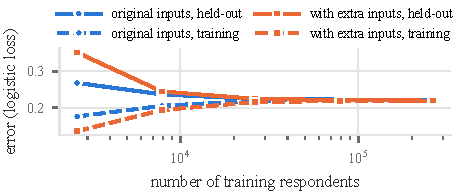
\includegraphics[width=\columnwidth]{fig_learning_curve}
  \vspace{-5mm}
  \caption{Logistic loss of logistic regression on the training data (dashed)
  and on held-out data (solid) as the training set grows.}
  \label{fig:lc}
\end{figure}

\subsection{From the Baseline to the Final Model}

With all the training data, logistic regression has the same logistic loss
on the people it learned from as on new people (Fig.~\ref{fig:lc}). The model
does not memorize the data. It is just too simple. Richer inputs should therefore help more than more data or a stronger
penalty, and Fig.~\ref{fig:ablation} confirms this. Squares and the products of 10 risk factors improve F1 by
\mbox{$0.004 \pm 0.002$}, more than turning every answer into yes/no indicators
achieves with twice as many inputs. Newton's method adds a little
more, and so do 20 risk factors instead of 10, which give 190 products
instead of 45.

The trees alone are slightly better than the best logistic regression,
partly because they use the empty answers. Of the people who answered the diabetes questions, 22\% are sick against
8.8\% overall. Averaging the two models adds $0.004 \pm 0.001$
over logistic regression alone, while a small neural network and deeper
trees did not help.

\begin{figure}[tbp]
  \centering
  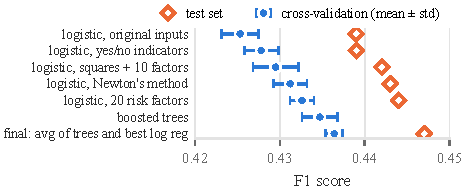
\includegraphics[width=\columnwidth]{fig_ablation}
  \vspace{-5mm}
  \caption{F1 score of each step towards the final model, in 5-fold CV
  (mean $\pm$ std) and on the test set. We never submitted the trees alone.}
  \label{fig:ablation}
\end{figure}

\subsection{A Leaking Column}

When we first gave the trees all the columns, F1 jumped by 0.012 on one part
of the data, far more than any other change. We traced 0.010 of it to a question about rehabilitation after a heart attack,
which is only asked to people who had one, so everyone who answered it is
sick.
A screening tool would never know this answer for someone undiagnosed, so we leave it out.

\section{Discussion}

Most of our gains are as small as the differences between the five parts of
the data. Comparing models part by part is what separated them from chance,
and the test scores confirmed the resulting ranking. The CV estimate is slightly optimistic, since
the cut-off and the number of trees were chosen on the same data that we
score, yet the test score is higher, which we cannot fully explain. All our
additions together gain only about 0.01 F1, so most of the performance comes
from logistic regression with a well-chosen cut-off. We also left some answers undecoded, such as the code 555 for ``never'' and
questions that mix answers per week and per month. Finally, the labels are diagnoses reported at the time of the survey, so the
model recognizes people who already have the disease rather than predicting
who will get it.

\section{Summary}

Logistic regression with a cut-off chosen for F1 is the best basic method. It is too simple rather than short of data, so we gave it
squares and products of known risk factors, and averaging it with gradient
boosted trees gave an F1 score of 0.436 in cross-validation and 0.447 on the
test set. Comparing all changes on the same data kept only consistent gains and found a question that leaked the answer.

\bibliographystyle{IEEEtran}
\bibliography{literature}

\end{document}
